In this section we present the results of a series of experiments we have conducted using AppScale and EAGER. We mainly focus
on the extra overhead imposed by EAGER on the application deployment process, as the number of deployed APIs and dependencies
grow. We also deploy a real-world API dataset (from ProgrammableWeb.com) on AppScale and EAGER, and evaluate how a large 
volume of API metadata can influence the behavior of EAGER.

\subsection{Performance on Stock AppScale without EAGER}
Before evaluating the performance overhead of EAGER, lets take a look at how long it takes to deploy an application on stock (unmodified)
AppScale. Table~\ref{tab:sample_apps} lists a number of sample applications along with their sizes and average deployment times on AppScale.
These applications have been chosen to represent a wide range of programming languages, application sizes and business domains. The average
deployment time and standard error values were computed over 3 readings.

\begin{table*}[ht]
\begin{center}
\begin{tabular}{| l | p{6cm} | l | l | l | }
\hline
Application & Description & Size & Deployment Time (s) & Std. Error\\ \hline
guestbook-py & A simple Python web application that allows users to post comments and view them & 16K & 22.13 & 0.34 \\ \hline
guestbook-java & A Java clone of the guestbook-python app & 52M & 24.18 & 0.09 \\ \hline
appinventor & A popular open source web application that enables creating mobile apps & 198M & 111.47 & 5.75 \\ \hline
coursebuilder & A popular open source web application used to facilitate teaching online courses & 37M & 23.75 & 0.30 \\ \hline
hawkeye & A sample Java application used to test AppScale & 35M & 23.37 & 0.27 \\ \hline
simple-jaxrs-app & A sample JAXRS app that exports 2 web APIs & 34M & 23.45 & 0.34 \\ \hline
dep-jaxrs-app & A sample JAXRS app that exports a web API and has one dependency & 34M & 23.72 & 0.32 \\ \hline
dep-jaxrs-app-v2 & A sample JAXRS app that exports 2 web APIs and has one dependency & 34M & 23.95 & 0.65 \\ \hline
\end{tabular}
\end{center}
\caption{Sample AppScale Applications}
\label{tab:sample_apps}
\end{table*}

Note that the smallest deployment time recorded on AppScale is 22.13 seconds. Also there's a clear correlation between the
size of the application, its average deployment time and the standard error observed. Larger applications take longer to deploy,
and exhibits a higher standard error. This is because larger applications take longer to be transferred over the network to the 
servers in the cloud. AppScale also archives and compresses application files for deployment, which takes extra
time.

We noticed at a very early stage that the extra overhead imposed by EAGER is much smaller compared to the overall application
deployment times observed in AppScale (100's of milliseconds compared to 10's of seconds). Therefore the EAGER overhead
is too small to be observed in a plot that illustrates overall application deployment time. This caused several difficulties when it
came to analyzing the results gathered from our experiments. The strong correlation between the
application size and the variance of the deployment time was another impediment in our evaluation.

Therefore, to avoid confusion and improve the accuracy and precision of our test results, we instrumented our experiments to
only record the extra time spent on EAGER. This way we were able to better analyze the impact of number of APIs and dependencies
on EAGER overhead. Hence, in the figures that follow we only present the additional time taken by EAGER during application
deployment process.

\subsection{EAGER Overhead by Application}

Figure~\ref{fig:overhead_by_app} illustrates the extra time taken by EAGER to validate and verify the sample AppScale applications.
These results were recorded on an EAGER deployment that didn't have any policies deployed, and without any prior
metadata recorded in the API metadata manager (that is, on a clean database).

\begin{figure}
\centering
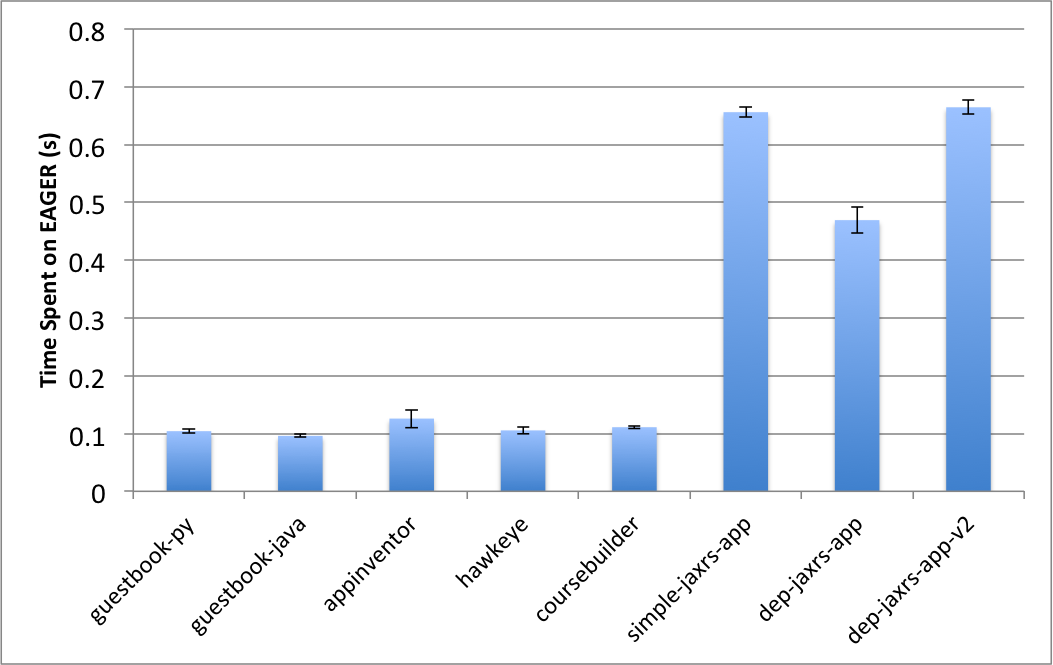
\includegraphics[scale=0.45]{overhead_by_app}
\caption{EAGER Overhead by Application}
\label{fig:overhead_by_app}
\end{figure}

Note that for the applications that do not export any web APIs, the overhead is negligibly small (around 0.1s). This is because EAGER
doesn't have to validate or record any metadata in the Metadata Manager for such applications. This implies that EAGER will not affect 
most existing AppScale apps, as long as their deployment time is concerned. For the applications that do 
export web APIs, however, EAGER has to record API metadata in the Metadata Manager, and they must be validated and published to 
the API gateway. As a result we see some extra overhead there. But even in these cases, the observed overhead is well under a second,
which is very small compared to the total application deployment time in AppScale (20+ seconds).

The overhead difference between dep-jaxrs-app-v1 and dep-jaxrs-app-v2 suggests that the EAGER overhead increases with the number
of APIs exported by an application. In the next section we will further evaluate this property.

\subsection{Impact of Number of APIs and Dependencies}

Figure~\ref{fig:overhead_by_apis} shows that the EAGER overhead grows linearly with the number of APIs exported by an application.
This is because, in our current implementation, we iterate through the APIs in the application sequentially, and record the associated metadata in the
Metadata Manager. Then EAGER also have to publish each API to the API Gateway, so that API consumers can invoke the APIs. Since
API Gateway is a separate component, this amounts to additional web service calls, one per API. Therefore, as more and more APIs are exported 
by an application, the overhead of application deployment process via EAGER grows linearly. 

\begin{figure}
\centering
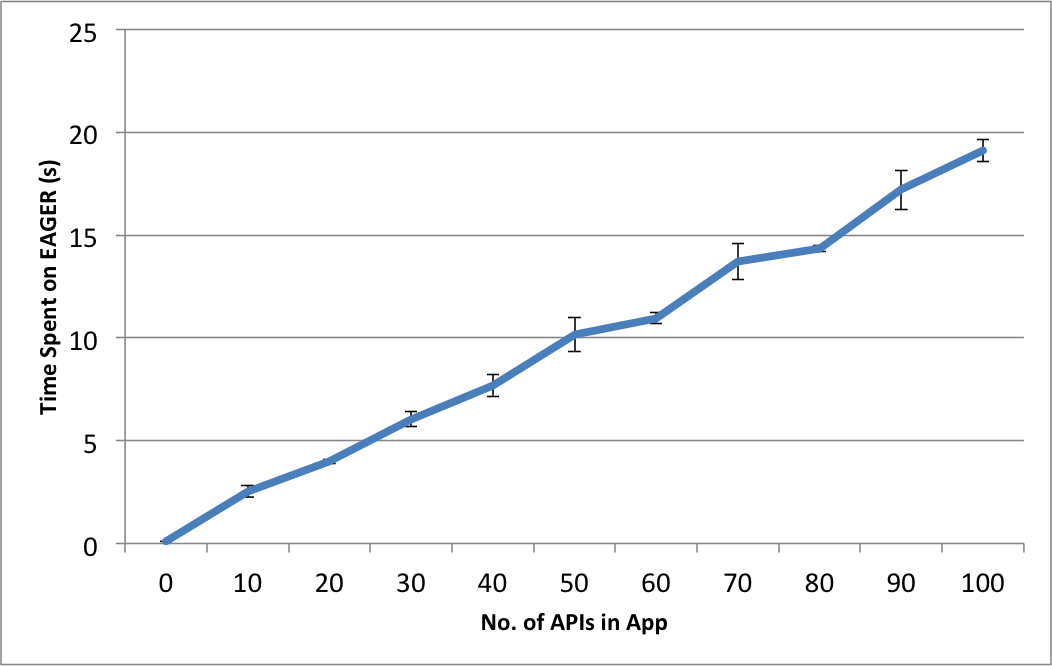
\includegraphics[scale=0.45]{overhead_by_apis}
\caption{EAGER Overhead vs. Number of APIs Exported by the Application}
\label{fig:overhead_by_apis}
\end{figure}

However, we believe that in practice this linear growth in overhead is not going to cause any serious issues for the application developers.
We expect most applications deployed in cloud to have a small to moderate number of APIs (1 to 10). According to our results, this is an 
extra overhead of 0.1-2.5 seconds, which is still very small compared to the total application deployment time of AppScale. Even in the
unlikely case of 50 APIs being exported by an application, we can only see a percentage overhead close to 30\%. It must also be noted, that
one may further improve the performance of EAGER by parallelizing the process of metadata recording and API publishing at the deployment
time. These tasks are largely independent of each other and hence there is nothing preventing them from being executed in parallel. That is,
if the developer attempts to deploy an application that exports $n$ APIs, EAGER can spawn $n$ threads where each thread will be responsible
for recording the metadata and publishing a single API.

Next, we analyze the EAGER overhead as the number of dependencies declared in an application grows. For this experiment, we first populate 
the EAGER Metadata Manager with metadata for 100 randomly generated APIs. Then we deploy an application on EAGER which exports a single
API and declares dependencies on the APIs that are already stored in the Metadata Manager. We vary the number of declared dependencies and
observe the additional overhead imposed by EAGER.

\begin{figure}
\centering
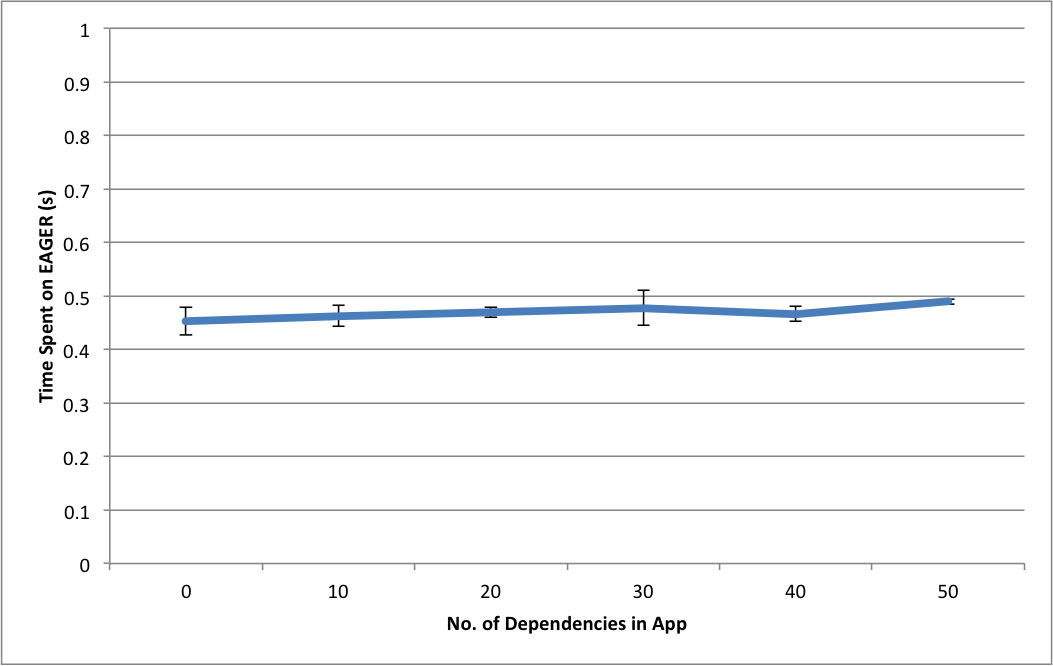
\includegraphics[scale=0.45]{overhead_by_deps}
\caption{EAGER Overhead vs. Number of Dependencies Declared in the Application}
\label{fig:overhead_by_deps}
\end{figure}

Figure~\ref{fig:overhead_by_deps} shows the results of the above experiment. According to that, the EAGER overhead is not significantly
influenced by the number of dependencies declared in an application. This is because in our current implementation, EAGER processes
all dependency related information via batch operations. That is, it sends all the dependencies declared in the application to the Metadata
Manager as a single batch. After validating and verifying the dependencies, Metadata Manager uses SQL batch operations to record
them in the database. As a result, the number of web service calls and database queries that originate due to varying number of dependencies
is fairly constant. This results in a reasonably constant overhead for all cases considered.

\subsection{Impact of Number of Policies}

So far all our experiments were conducted without any active governance policies in the system. In this section we report how EAGER overhead
varies with the number of policies deployed in the PaaS. 

We understand that the overhead of policy validation is largely dependent
on the actual content (Python code) that's contained in the policies. Since users are free to include any Python code they see fit (as long as it
falls in the accepted subset) in a policy file, evaluating a given policy could take an arbitrary amount of time. Therefore, in this experiment, our
goal is to evaluate the extra overhead incurred by simply having many policy files to execute. We intentionally keep the content of the policies
small and trivial. We create a policy file that runs following assertions:
\begin{enumerate}
\item Application name must start with an upper case letter
\item Application must be owned by a specific user (admin@test.com)
\item All API names must start with upper case letters
\end{enumerate}
We create many copies of this initial policy file to vary the number of policies deployed. Then we evaluate the overhead of policy validation
on two of our sample applications (guestbook-py and simple-jaxrs-app). 

\begin{figure}
\centering
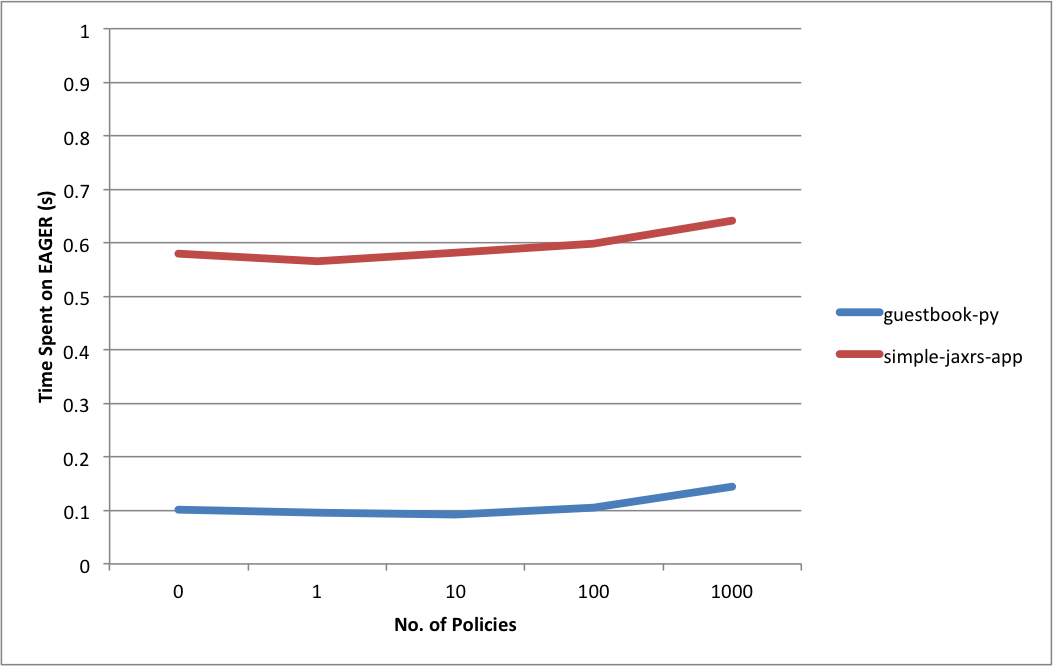
\includegraphics[scale=0.45]{overhead_by_policies}
\caption{EAGER Overhead vs. Number of Policies}
\label{fig:overhead_by_policies}
\end{figure}

Figure~\ref{fig:overhead_by_policies} shows how the number of active policies impact the EAGER overhead. Interestingly, having many
different policy files have very little influence on the EAGER overhead. It is only when the active policy count approaches 1000 that we
can see a noticeable increase in the overhead. Even then, the increase in deployment time is under 0.1 seconds. 

This behavior is due to the fact that EAGER loads policy content into memory at system
startup (or when a new policy is deployed), and executes them from memory each time an application is deployed. Since policy files are 
typically small (at most a few kilobytes), this is a viable option. The overhead of validating the simple-jaxrs-app is higher than that of the
guestbook-py application because, unlike guestbook-py, simple-jaxrs-app exports web APIs. This means the third assertion listed earlier
needs to be executed for simple-jaxrs-app. In our test policy file this particular assertion has been implemented as a loop that iterates through 
all APIs exported by the application which incurs some extra cost to execute.

Above results indicate that EAGER scales well to hundreds of policies. That is, there is no significant overhead associated with simply having
a large number of policy files. However, as mentioned earlier, the content of a policy can have a significant influence on the overhead
 caused by EAGER.
 
\subsection{Scalability}
Next we evaluate how EAGER scales when a large number of APIs are deployed in the cloud. In this experiment, we populate the EAGER
Metadata Manager with a varying number of APIs, and then attempt to deploy various sample applications on AppScale. We also create
random dependencies among the APIs recorded in the Metadata Manager to make the setting more realistic.

\begin{figure}
\centering
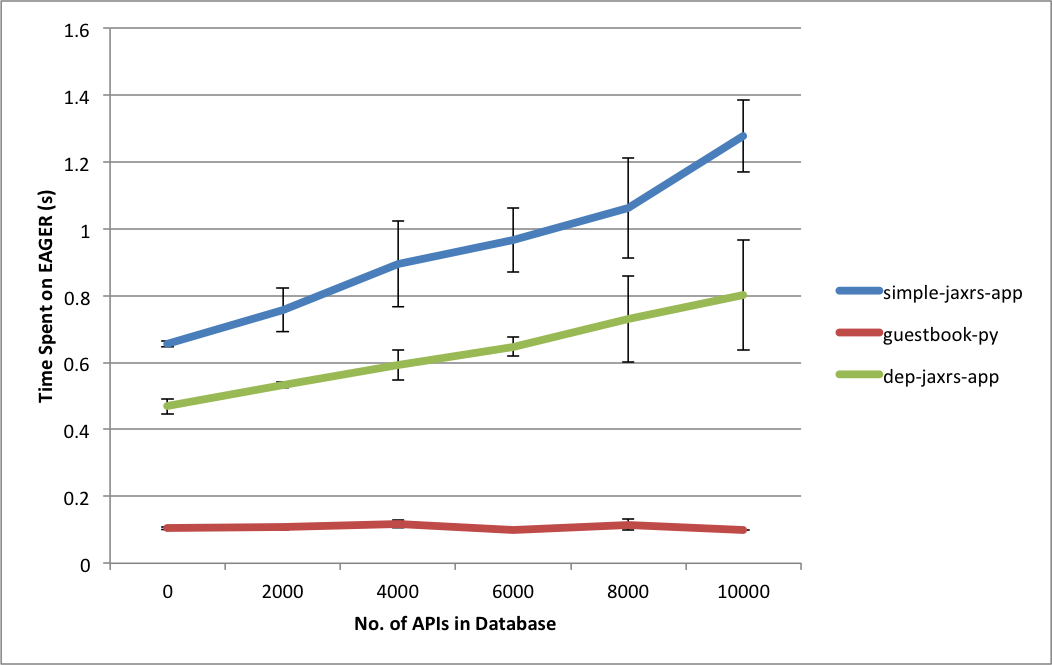
\includegraphics[scale=0.45]{scalability}
\caption{EAGER Overhead vs. Number of APIs in Metadata Manager}
\label{fig:scalability}
\end{figure}

Figure~\ref{fig:scalability} shows that the deployment overhead of the guestbook-py application is not impacted by the growth of metadata
in the cloud. Recall that guestbook-py does not export any APIs nor it declares any dependencies. Therefore the deployment process of
the guestbook-py application has minimal interactions with the Metadata Manager. Based on this result we may conclude that applications that
do not export web APIs are not significantly affected by the accumulation of metadata in EAGER.

Both simple-jaxrs-app and dep-jaxrs-app are
somewhat affected by the volume of data stored in EAGER Metadata Manager. Since these applications export web APIs that must be 
recorded and validated by the Metadata Manager, the explosion of metadata has an increasingly higher impact on them. This degradation 
of performance is primarily due to the slow query performance of the RDBMS engine (MySQL) as the database size grows. The simple-jaxrs-app
is affected more than dep-jaxrs-app by this performance drop, because simple-jaxrs-app exports two APIs compared to the single API exported 
by dep-jaxrs-app. However, on a more positive note, the growth
in overhead is linear to the number of APIs deployed in the cloud which indicates a fairly good scalability trait. Also it is encouraging to see that
even after deploying 10000 APIs, the overhead of simple-jaxrs-app has only been increased by about 0.5 seconds, which is very small compared
to the total deployment time of the application.

Another interesting attribute to notice in figure~\ref{fig:scalability} is the growing amount of variance in the overhead as the number of APIs in the cloud grows.
We believe this is due to the increasing variability of database query performance and the data transfer performance as the size of the 
database increases.

Overall, we can conclude that EAGER scales well to 1000's of APIs. This is a very positive result, as today's popular API registries (e.g. ProgrammableWeb.com) 
place the total number of APIs in the Internet somewhere in the range of 10000 to 15000. If further scalability is required, we can leverage the past and ongoing
work from the database community, and use a faster, and more scalable database engine (e.g. a NoSQL engine) to implement the
EAGER Metadata Manager rather than using a simple RDBMS.

\subsection{Experimental Results with a Real-World Dataset}
Finally, we explore how EAGER operates when loaded with a real-world dataset with real API metadata and dependency information. For this, we 
crawl the ProgrammableWeb.com registry and extract metadata regarding all the registered APIs and mashups. By the time we conducted
this experiment, there were 11095 APIs and 7227 mashups registered in ProgrammableWeb. Each of the mashups depend on one or more APIs.

We started by adding all 11095 APIs to the EAGER Metadata Manager. Then we also registered each of the mashups as APIs in EAGER. We used the
mashup-API dependency information extracted from ProgrammableWeb to register dependencies among the APIs in EAGER. This resulted in a 
dependency graph of 18322 vertices (APIs and mashups) and 33615 edges. With EAGER pre-populated with all this metadata, we then deploy
some of our sample applications on AppScale to measure the deployment overhead caused by EAGER.

\begin{figure}
\centering
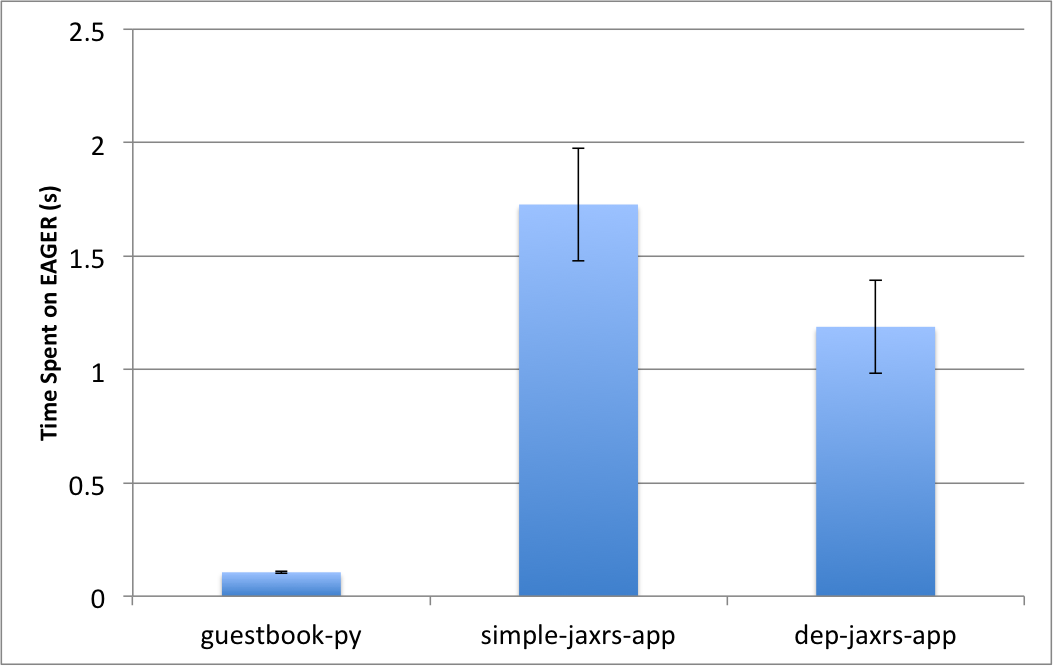
\includegraphics[scale=0.45]{pweb_sample_overhead}
\caption{EAGER Overhead When Deploying on ProgrammableWeb Dataset}
\label{fig:pweb_sample_overhead}
\end{figure}

As shown in figure~\ref{fig:pweb_sample_overhead}, the guestbook-py app is not significantly impacted by having a large dependency graph. This is
expected since guestbook-py doesn't export any web APIs. The applications that do export web API, and hence have to interact with the Metadata
Manager register a slightly higher deployment overhead. But the highest overhead observed is under 2 seconds, which is still very small compared
to the total application deployment time (20+ seconds). The simple-jaxrs-app shows a higher overhead than dep-jaxrs-app because it exports one
additional web API than dep-jaxrs-app. 

All three sample applications considered in the above experiment do not declare dependencies on any of the APIs or mashups in the ProgrammableWeb
dataset. The dep-jaxrs-app does declare a dependency, but that is on an API exported by simple-jaxrs-app. To see how the deployment time is impacted
when applications take dependencies on other APIs registered in EAGER, we deploy a test application that declares random dependencies on APIs
registered in EAGER Metadata Manager (this application also exports a web API). We change the declared dependency count between 
10 and 50 and also redeploy the application multiple times.
In one set of experiments, we run a deployment script that randomly modifies the declared dependencies at each redeployment. In another set of 
experiments, we redeploy the application without further randomizing the declared dependencies.

\begin{figure}
\centering
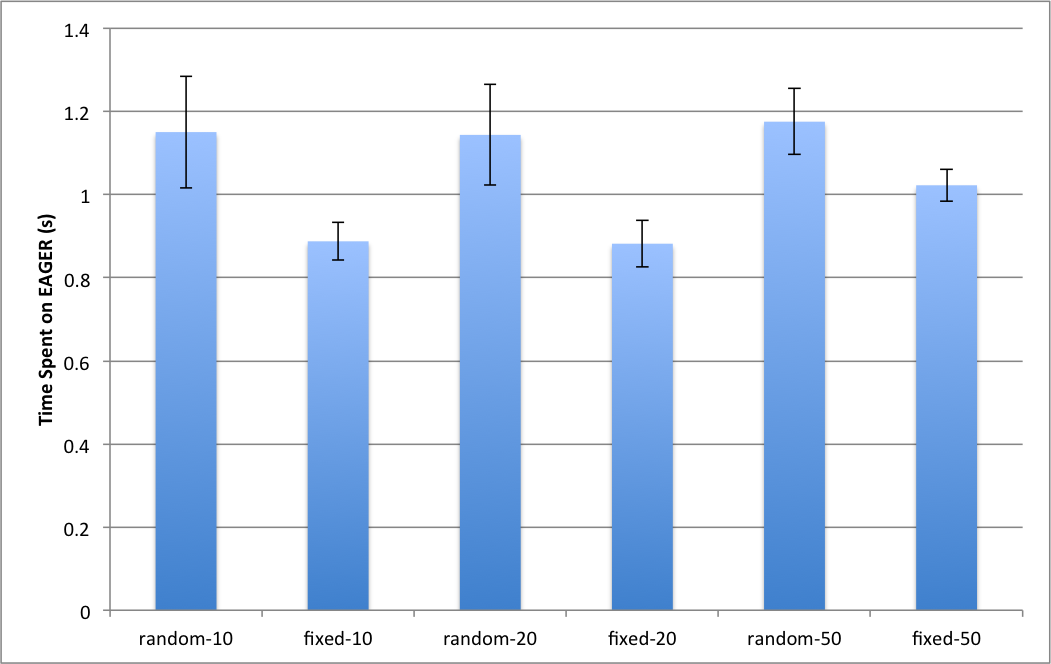
\includegraphics[scale=0.45]{pweb_random_overhead}
\caption{EAGER Overhead When Deploying on ProgrammableWeb Dataset with Dependencies}
\label{fig:pweb_random_overhead}
\end{figure}

Figure~\ref{fig:pweb_random_overhead} illustrates results from both sets of experiments. Columns labeled as ``random'' indicate the average overhead
computed across 3 redeployments, where the declared dependencies were randomized prior to each redeployment. Columns labeled as ``fixed'' show
the average overhead calculated across 3 redeployments, where the dependency declaration was kept fixed across redeployments. The numeric value
in each label indicates the number of dependencies declared.

Interestingly, having many dependencies do not have a big impact on the overhead. This is inline with our observations in figure~\ref{fig:overhead_by_deps}.
It is encouraging to see that the same property holds when the Metadata Manager is loaded with over 18000 entries, that has real-world dependency
relationships among them. The largest overhead observed is under 1.2 seconds, which is significantly smaller than the total deployment overhead of AppScale.
Also it is interesting to see that, whenever the dependency declaration was kept fixed, the overhead is slightly smaller. This is because our prototype caches
the edges of the dependency tree that have been read, which makes immediate redeployments go faster.